\documentclass[12pt]{article}

\usepackage{../Ceyhun}
\usepackage{../amsTurkish}
\usepackage{sectsty}

\begin{document}

	\hPage{ceyhun-048}

	\underline{2.1 Çakışım ile ilgili tanım matrisleri}

	olmayan yalnız iki terim vardır. \\

	\begin{definition}
	
	Çakışım matrisi ${\LARGE \overline{P}}$ nin, herhangi bir dizeğinin atılması ile elde edilen {\LARGE P} matrisine, \underline{\textit{indirgenmiş çakışım matrisi}} denir. \\

	\end{definition}

	Çizge üzerinde tanımlanabilecek en önemli matris olan çakışım matrisinin ayrıntılı incelenmesini 3. Bölüme bırakacağız. \\

	\begin{definition}

	Düğüm ve ayrıtları arasında, çakışım ilişkisinin sakınıldığı, 1:1 bir karşıdüşme olan çizgelere \underline{\emph{eşyapılı} çizge} denir. \\

	\end{definition}

	Tanım 2.1.3 ten, eşyapılı çizgeler için çakışım matrislerinin eşit olacak biçimde yazılabileceği gözden kaçmamalıdır. Şekil 2.1.1 deki $\LARGE{Ç_{1}}$ ve $\LARGE{Ç_{2}}$ çizgelerinin düğüm ve ayrıtları arasında,

	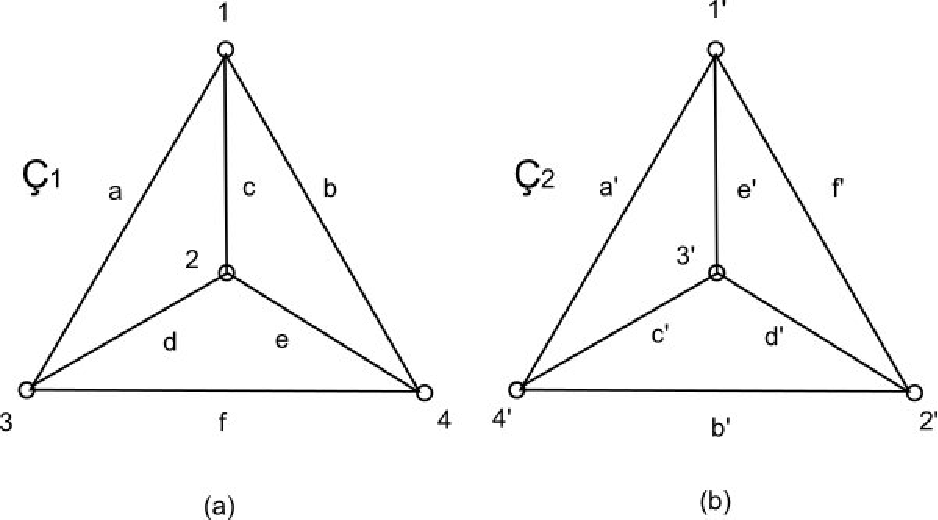
\includegraphics{images/ceyhun-048-fig01.pdf} %figure

	Şekil 2.1.1 Eşyapılı çizgeler.

\end{document}

